\documentclass[14pt]{beamer}

% Presento style file
\usepackage{config/presento}

% custom command and packages
\input{config/custom-command}

% Information
\title{Guess the Package!}
\subtitle{A Predictive Classification Model}
\author{Yashi Srivastava}
\institute{TalentSprint WE}


\begin{document}

% Title page
\begin{frame}[plain]
\maketitle
\end{frame}

% sections in the presentation
\begin{frame}{Aim}
\renewcommand{\labelitemi}{$\square $}
 \begin{fullpageitemize}
  \item Identifying features influencing salary
  \pause
  \item Building a classifier for predicting range of probable package
 \end{fullpageitemize}
\end{frame}
\begin{frame}{Languages/Libraries Used}
\pause
\renewcommand{\labelitemi}{$\square $}
 \begin{fullpageitemize}
  \item Python3 
  \\~\
  \item scikit learn, pandas, matplotlib
 \end{fullpageitemize}
\end{frame}
\begin{frame}{Dataset Description}
\pause
\renewcommand{\labelitemi}{$\square $}
 \begin{fullpageitemize}
  \item AMCAT AMEO Dataset 
  \item 38 features 
  \item 4000 tuples 
  \item 11 features of string data-type
 \end{fullpageitemize}
\end{frame}

\begin{frame}{Work-Plan}
\pause
Planned tasks, each for 2 days- 
\\~\
\renewcommand{\labelitemi}{$\square $}
 \begin{fullpageitemize}
  \item Data - Preprocessing
  \item Feature Reduction and Feature Scaling 
  \item Comparing various classification algorithms 
 \end{fullpageitemize}
\end{frame}
\begin{frame}{Data - Preprocessing}
\pause
\renewcommand{\labelitemi}{$\square$}
 \begin{fullpageitemize}
  \item Board of schooling
  \item Segregating job city by code is data approach. 
  \item Dealing with non-numeric columns of dataset
  \item Salary segregation in two classes
 \end{fullpageitemize}
\end{frame}
\begin{frame}{Segregating Salary}
Classes made on the boundary of 3 Lakhs.
\pause
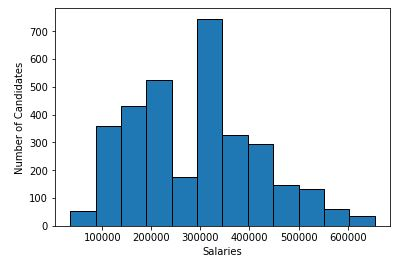
\includegraphics[]{salaryDistribution.JPG}
\end{frame}
\begin{frame}{Feature Reduction}
\pause
\renewcommand{\labelitemi}{$\square$}
 \begin{fullpageitemize}
  \item Reducing 8 columns of  technical score to 3 columns
  \item Dropping columns which had no effect on the salary.
 \end{fullpageitemize}
\end{frame}
\begin{frame}{Outlier Detection}
\pause
\renewcommand{\labelitemi}{$\square$}
 \begin{fullpageitemize}
  \item Using 1st and 3rd quartiles
  \item From 3999 rows, 723 rows were dropped.
  \item Upper bound for salary was 6.55 lakhs
 \end{fullpageitemize}
\end{frame}
\begin{frame}{Applying Machine Learning}
\pause
\renewcommand{\labelitemi}{$\square$}
 \begin{fullpageitemize}
  \item Split data into train, test and validation
  \item Models were trained on a number of algorithms, and results were compared.
 \end{fullpageitemize}
\end{frame}
\begin{frame}{Comparing different algorithms}
\pause
 \begin{fullpageitemize}
 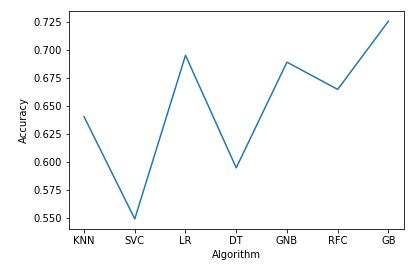
\includegraphics{algorithmComparison.JPG}
 \end{fullpageitemize}
\end{frame}
\begin{frame}{Challenges}
\pause
\renewcommand{\labelitemi}{$\square$}
 \begin{fullpageitemize}
  \item A lot of missing values 
  \item Dealing with semantically similar but differently spelled strings 
 \end{fullpageitemize}
 \end{frame}
 \begin{frame}{Further Work}
\pause
\renewcommand{\labelitemi}{$\square$}
 \begin{fullpageitemize}

   \item Improving accuracy beyond 72\% of Gradient Boosting Algorithm.
  \item Consuming the model

 \end{fullpageitemize}
 \end{frame}
 \begin{frame}{}
 \centering
            \Huge\bfseries
        \textcolor{orange}{Discussions}
\end{frame}
\end{document}